\appendix
\section{The use of generative AI (ChatGPT)}
OpenAI's ChatGPT interface, powered by the GPT-4 large language model, was used to create some code.
\subsection{\_inverse\_triangluar\_matrix\ method}
This method is used to calculate the inverse of R in my method that computes the NLML in my FITC sparse GP approximation.
It was generated using ChatGPT using the prompt: ``Write a Python function named \_inverse\_upper\_triangular that calculates the inverse of an upper triangular matrix in a faster and more numerically stable way than the standard np.linalg.inv function``.
The output is provided in Figure~\ref{fig:chat-iut}.:
\begin{figure}[htbp]
    \centering
    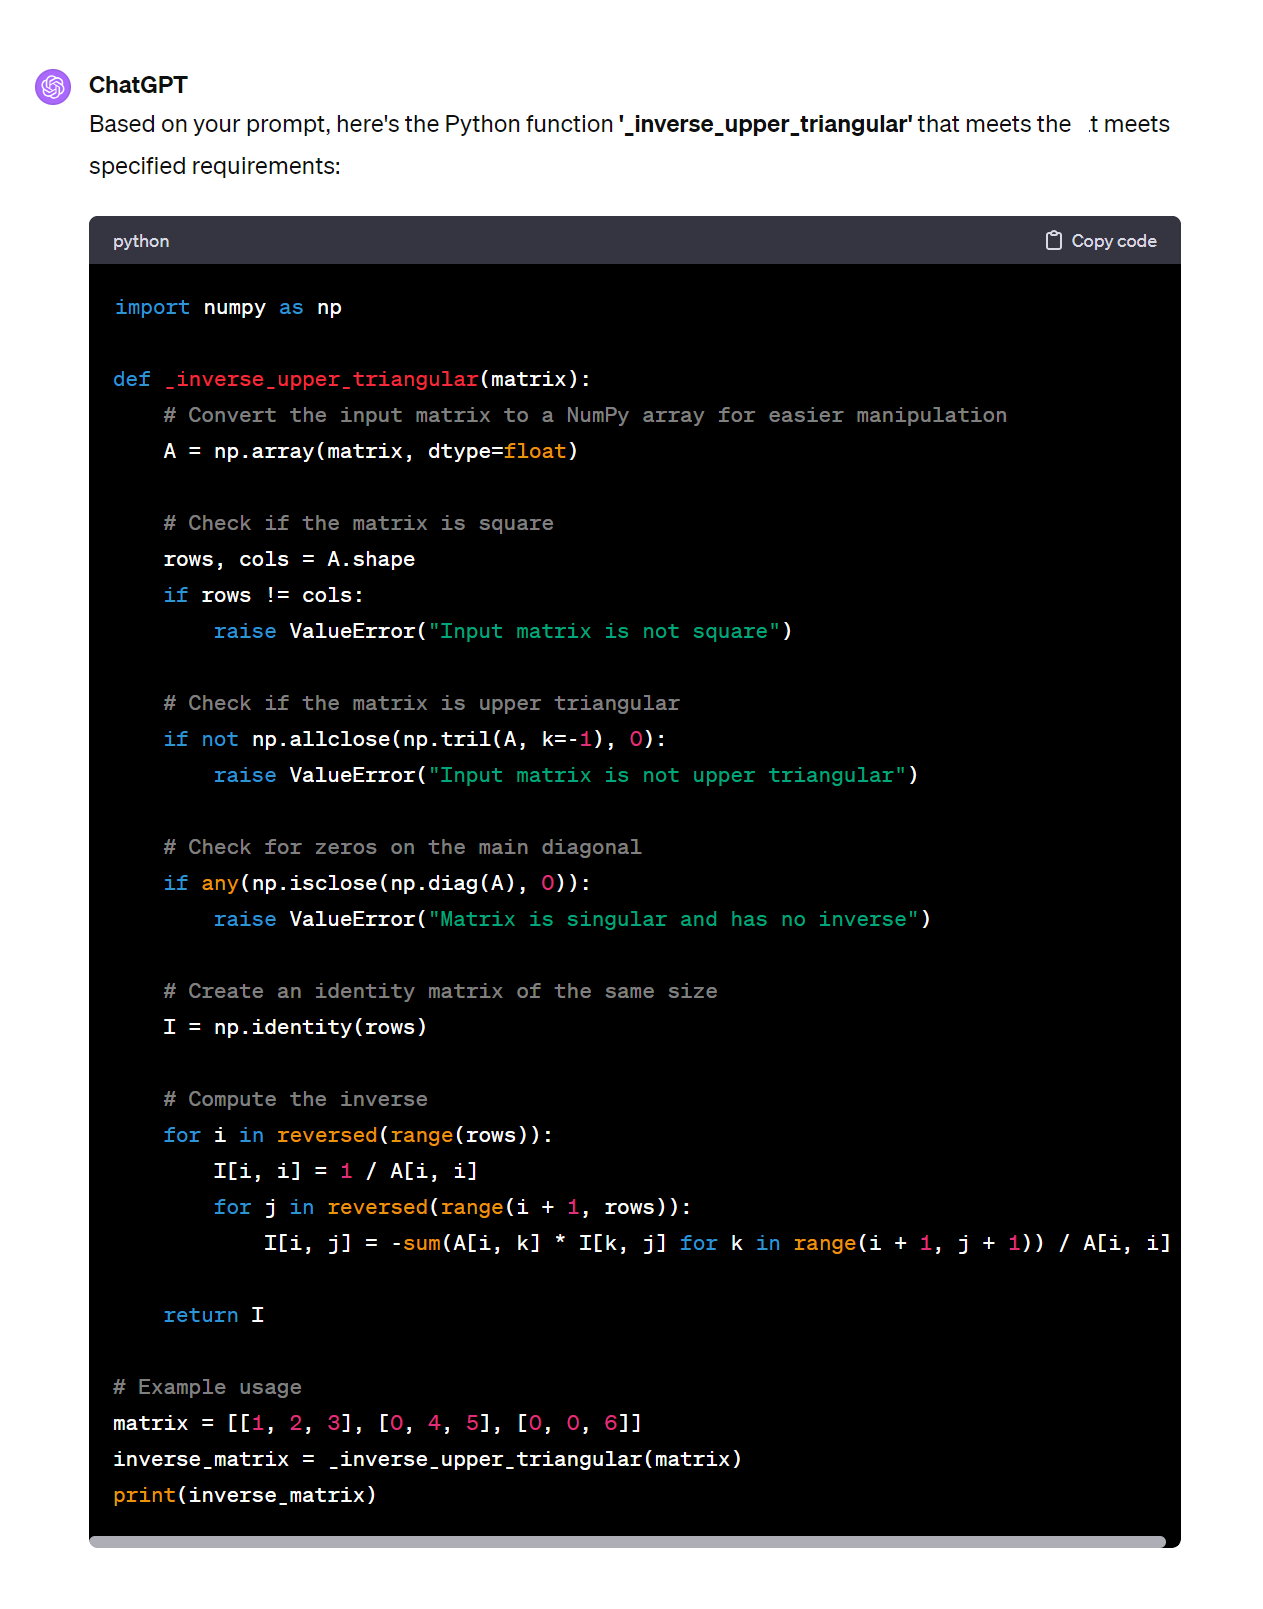
\includegraphics[width=1\linewidth]{figures/chat-iut/chat-iut.png}
    \caption{ChatGPT output providing a function used to inverse an upper triangular matrix in a faster and more numerically stable way}
    \label{fig:chat-iut}
\end{figure}



After this was generated, it was modified slightly to make it work in my FITC class.
Firstly, it was made a method instead of a function by adding ``self`` to the inputs.
Secondly, the output was transformed into a np.array type which is expected for the subsequent code.
The resulting method is provided below:

\FloatBarrier

\begin{lstlisting}[language=Python]
    def _inverse_upper_triangular(self, matrix):
        # Convert the input matrix to a NumPy array for easier manipulation
        A = np.array(matrix, dtype=float)

        # Check if the matrix is square
        rows, cols = A.shape
        if rows != cols:
            raise ValueError("Input matrix is not square")

        # Check if the matrix is upper triangular
        if not np.allclose(np.tril(A, k=-1), 0):
            raise ValueError("Input matrix is not upper triangular")

        # Check for zeros on the main diagonal
        if any(np.isclose(np.diag(A), 0)):
            raise ValueError(
                "Matrix is singular and has no inverse")  # Changed from return None for consistency

        # Create an identity matrix of the same size
        I = np.identity(rows)

        # Compute the inverse
        for i in reversed(range(rows)):
            I[i, i] = 1 / A[i, i]
            for j in reversed(range(i + 1, rows)):
                I[i, j] = -sum(A[i, k] * I[k, j] for k in range(i + 1, j + 1)) / A[i, i]

        return np.array(I.tolist())
\end{lstlisting}

This was proven to work by writing a unit test:

\FloatBarrier

\begin{lstlisting}[language=Python]
    def test__inverse_upper_triangular(self):
        obj = GP_NLL_FITC(1, 2, 3, 4, 5, 6)

        # Upper triangular matrix
        matrix = np.array([
            [2, 3, 1],
            [0, 4, 5],
            [0, 0, 7]
        ])

        start_time = timer.time()

        result = obj._inverse_upper_triangular(matrix)

        end_time = timer.time()
        elapsed_time = end_time - start_time
        print(f"The _inverse_upper_triangular func ran in {elapsed_time} seconds")

        start_time = timer.time()

        correct = np.linalg.inv(matrix)

        end_time = timer.time()
        elapsed_time = end_time - start_time

        print(f"The np.linalg.inv func ran in {elapsed_time} seconds")
        debug_print(f"result = {result}")
        debug_print(f"correct = {correct}")
        debug_print(f"difference = {result - correct}")

        assert np.allclose(result, correct, atol=1E-5, rtol=1E-5)

        # Another upper triangular matrix with different values
        matrix2 = np.array([
            [-1.9883, 2.0, 3.0],
            [0, -9.4199, 4.0],
            [0, 0, 1.7969]
        ])

        start_time = timer.time()
        result2 = obj._inverse_upper_triangular(matrix2)
        end_time = timer.time()

        elapsed_time = end_time - start_time
        print(f"The _inverse_upper_triangular func ran in {elapsed_time} seconds")

        start_time = timer.time()
        correct2 = np.linalg.inv(matrix2)
        end_time = timer.time()

        elapsed_time = end_time - start_time
        print(f"The np.linalg.inv func ran in {elapsed_time} seconds")
        debug_print(f"result2 = {result2}")
        debug_print(f"correct2 = {correct2}")
        debug_print(f"difference2 = {result2 - correct2}")

        assert np.allclose(result2, correct2, atol=1E-5, rtol=1E-5)
\end{lstlisting}


This compared the result calculated by the method with an expected result calculated using the standard \texttt{np.linalg.inv} function for the two different input matrices.
If they were the same within both a relative and absolute tolerance of $1E-5.$

The unit test passed, showing that the function inverses the matrix correctly, however, it wasn't necessarily faster than the standard \texttt{np.linalg.inv} function.
The inverse of the first matrix was calculated in $0.000246$ and $0.001368$ seconds using \texttt{\_inverse\_upper\_triangular} and \texttt{np.linalg.inv} methods respectively, whereas the inverse of the second matrix was calculated in $0.000312$ and $0.00005$ seconds respectively.
This indicates that the fastest method depends on the input matrix, which is likely true for larger matrices also since both functions are of the $O(n^3)$ for an $n \times n$ matrix.
However, the \texttt{\_inverse\_upper\_triangular} function will be more numerically stable and memory efficient because it is taking adavantages of the fact that the input matrix is upper triangular which allows the inverse to be found by back substitution instead of it being computed naively.
\FloatBarrier

\subsection{Figures for the report}
\subsubsection{Cumulative Distribution Function}
Put prompt and output
